\documentclass[a4paper,10pt]{article}

%\usepackage[latin1]{inputenc}
\usepackage{algorithm}
\usepackage{algorithmic}
\usepackage{amsmath}
\usepackage{amsfonts}
\usepackage{amssymb}
\usepackage{graphicx}
\usepackage{epsfig} % for postscript graphics files
\usepackage{color}

%%%%%% Latex Configuration
% tips taken from http://dcwww.camd.dtu.dk/~schiotz/comp/LatexTips/LatexTips.html
\renewcommand{\topfraction}{0.85}
\renewcommand{\textfraction}{0.1}
\renewcommand{\algorithmiccomment}[1]{// #1}
%%%%%
\long\def\symbolfootnote[#1]#2{\begingroup%
\def\thefootnote{\fnsymbol{footnote}}\footnote[#1]{#2}\endgroup}

\newtheorem{definition}{Definition}
\newtheorem{theorem}{Problem}

\begin{document}

\begin{titlepage}
\begin{center}



\includegraphics[width=0.9\textwidth]{images/logo.jpg}\\[1cm]
\textsc{\LARGE Bar Ilan University}\\[1.5cm]
\textsc{\Large M.Sc Proposal}\\[0.5cm]
%\hrule \\[0.4cm]
%{\huge \bfseries Speeding Frontier-Based Exploration by
%Using Semantic Labeling}\\[0.4cm]
%\hrule \\[1.5cm]

\hrule
{ \vspace{2 mm} }
{ \huge \bfseries Speeding Frontier-Based Exploration by
Using Semantic Labeling}
{ \vspace{3 mm} }
\hrule
{ \vspace{8 mm} }
% \author{Matan Keidar\\
% advised by Gal A. Kaminka\\
% The MAVERICK Group, Computer Science Department\\
% Bar Ilan University\\
% Ramat Gan, Israel 52900\\
% \tt\small matankdr@gmail.com

%author and supervisor
\begin{minipage}{0.4\textwidth}
\begin{flushleft} \large
\emph{Author:}\\
Matan Keidar 

\end{flushleft}
\end{minipage}
\begin{minipage}{0.4\textwidth}
\begin{flushleft} \large
\emph{Supervisor:} \\
Gal A. Kaminka
\end{flushleft}
\end{minipage}


\vfill


\large{The MAVERICK Group, Computer Science Department\\
Bar Ilan University\\
Ramat Gan, Israel 52900\\
\tt\small matankdr@gmail.com}

\vfill

\today

\end{center}
\end{titlepage}

%opening
\title{Speeding Frontier-Based Exploration by Using
Semantic Labeling}
\author{Matan Keidar\\
advised by Gal A. Kaminka\\
The MAVERICK Group, Computer Science Department\\
Bar Ilan University\\
Ramat Gan, Israel 52900\\
\tt\small matankdr@gmail.com
}

\tableofcontents
\maketitle

\section{Introduction}
The problem of exploring an unknown territory is one of the fundamental
problems in robotics. The goal of exploration is to gain as much new information
as possible of the environment within a short time. Applications of efficient
exploration include search and rescue, planetary exploration
\cite{apostolopoulos2001robotic} and military uses \cite{hougen2000miniature}.


% We propose to speed up the exploration process by dealing with 2 aspects: an
% improved frontier detection algorithm () Section

This thesis proposal deals with making the exploration process faster.
Frontier-Based exploration is the most common approach for solving the
exploration problem. However, frontiers detection is very hard. We propose a
new frontier detection algorithm (section
\ref{section:FrontierBasedExploration}). In Section
\ref{section:SemanticLableing} we propose to use semantic labels in
order to speed up the exploration process. 

% The main motivation of exploration is letting the robot navigate in its
% environment without any human intervention (loading pre-prepared obstacle map in
% advance). Moreover, . Therefore, exploration
% is not a mapping problem, which outputs a map that contains every part of the
% environment.

% Many robots can navigate using maps. However, few robots can
% analyze their environment and generate a map. Usually, human intervention is necessary in order to map the territory in advance, providing a-priori information to the robot (i.e. , the exact locations of obstacles for metric maps or connectivity graph between open regions for topological maps). Applying exploration techniques can free the robots from the above limitation.



% Using a team of robots has advantages over the use of a single robot. The reason
% is that a team of coordinated robots can accomplish the exploration
% task much faster than a single robot. Moreover, it can also be more robust to
% failures.
% The problem of using a team is that two robots might interfere with each other
% (i.e, block the passage or accidentally map each other as obstacles \cite{simmons_coordination_2000})




\subsection{Frontier-Based Exploration}
\label{section:FrontierBasedExploration}

The most common approach to exploration is based on \emph{frontiers}. 
A frontier is a segment that separates known (explored) regions from unknown
regions. Thus, frontiers are important targets for exploration. Yamauchi
\cite{yamauchi_frontier-based_1997, yamauchi_frontier-based_1998} was the
first to show a frontier-based exploration strategy.

However, frontiers are hard to calculate. Most of frontier detection methods
are based on edge detection and region extraction techniques from computer
vision. The meaning of the above fact is that in order to detect the frontiers,
each time we have to process the entire world map data.

We propose an incremental approach for frontier detection (Algorithm
\ref{alg:IncrementalFrontierDetector}). Our proposed algorithm does not have to
scan the entire world data for detecting frontiers. It processes only not
previously scanned regions.

\begin{figure}
 \centering
 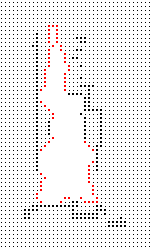
\includegraphics[width=0.4\columnwidth,keepaspectratio]{images/detect-edges.png}
 \caption{Frontiers detection example (image was taken from 
 \cite{_frontier-based_????}).}
 \label{fig:Frontiers}
\end{figure}

%An outline of the exploration process can be described as follows:




\subsection{Semantic Labeling}
\label{section:SemanticLableing}

The exploration process can also be improved by exploiting a-priori
knowledge of the explored environment. In general, exploration of
indoor environments like office building can exploit the fact that most
likely, explored objects are rooms which are connected by corridors. In
addition, rooms will probably consist of 4 walls, one door and 4 corners
with 90 degrees angles. The exploring robot can exploit the
above features to improve its navigation (i.e. speed).

In addition, better reasoning about world objects (such as doors,
rooms, corridors) can improve the communication between the robot and its
operator. Operator-robot communication can be more naturally due to applying
\emph{semantic labels} on world objects. For instance, the robot can accept
commands such as: ``Search behind the desk that is located in the second room from the right side
of this corridor``. This capability is called \emph{Semantic Labeling} which
involves applying semantic information to the environment.

We propose several heuristics which use such semantic information to enhance
the speed of the exploration process not only by performing a smarter
environment scan, but also reduce interruptions to the operator. 

\section{Background and Related work}
%2-3 pages
\subsection{Frontier-Based Exploration}

The problem of exploring an unknown environment with a single or multi mobile
robots has been concerning many authors. There are two aspects that have to be
taken care of:
\begin{itemize}
  \item Deciding on next target to be explored
  \item Coordinating the team members in order to minimize overlaps
\end{itemize}

An outline of the exploration process is described in Algorithm
\ref{alg:ExplorationOutline}.

\begin{algorithm}%[H] %TODO: check if should remove this [H]
\caption{Exploration Outline}
\label{alg:ExplorationOutline}
\begin{algorithmic}[1]
\WHILE{exists any unknown territory}
\STATE{allocate each robot a new set of targets}
\STATE{each robot visits its target and includes the new data obtained from its
sensors}
\ENDWHILE
\end{algorithmic}
\end{algorithm}

Yamauchi \cite{yamauchi_frontier-based_1997, yamauchi_frontier-based_1998}
developed a method that can be used by a team of robots. The robots explore an
unknown environment and exchange information with each other when they get new
sensor readings. As a result, the robots build a common map (occupancy grid) in
a distributed fashion. The map is always being updated until no new readings are
available. This work also introduces the notion of a \emph{frontier}. In
this method, each robot is heading to the \emph{centroid}\symbolfootnote[1]{The
centroid of a finite set of k points ${x_1, x_2, \ldots, x_k} \in \mathbb{R}^n$ is defined by:
$$ C = \frac{1}{k} \sum_{j=1}^{k} {x_j}$$, }, the center of mass, 
of the closest \emph{frontier}. In this
method, all robots navigate to their target independently while they share a
common map. Although Yamauchi's method is robust for disconnections, it is
clearly not optimal because there is no coordination between the team members.
Team members might cover the same area or even interfere with each other and
map each other as an obstacle. 

% this paper was published BEFORE the next one (simmons_coordinatino_2000)
Burgard et al. \cite{burgard_collaborative_2000} presented a probabilistic
approach for coordinating a team of robots. Their method considers the
trade-off between the costs of reaching a target and the utility of reaching
that target. In order to minimize overlaps between team members, they defined
the utility of a target by the size of the unexplored area that can be covered
by the robot's sensors upon reaching that target. Whenever a target point is
assigned to a specific team member, the utility of the unexplored area visible
from this target position is reduced for the other team members. This way a team
of multiple robots can minimize overlapping in the coverage area. Their method
is centralized in contrast to our proposed work.

Burgard et al. \cite{simmons_coordination_2000} proposed to assign a
target destination to each robot in a way that that maximizes the expected
map knowledge over time.
%In practice, the computation of the optimal solution
%is intractable. 
They proposed a bid-based heuristic. Each robot estimates
its utility and cost until arriving various targets. According to this
calculation, each robot creates bids. After receiving all bids, a central
agent assigns a target to each robot considering minimization of the overlapping
coverage of the team members. 

Ko et al. \cite{ko_practical_2003} presented a decision-theoretic approach to
the mapping and exploration problem. Their approach uses an adopted version of
particle filters to estimate the position in the other robot's partial map.

Lau \cite{lau_behavioural_2003} presented a behavioral approach.
The authors assume that all team members start from a known
location. The team members follow the behavior and spread in the
environment while updating a shared map. The coordination of team
members is achieved by using potential fields. Moreover, frontier-based path
planning is used to avoid convergence to local minima.

Sawhney et al. \cite{sawhney_fast_2009} presented an exploration
method for both 2D and 3D environments. They showed a novel visibility
per-time metric that is being used by the exploration algorithm. 
Their method covers nearly the same number of points like other metric method
that can be found in literature. However, the time length of the paths is
smaller. The outcome is reduced exploration time. 

Bouraqadi et al. \cite{bouraqadi_flocking-based_????} proposed a flocking based
approach for solving the exploration problem. Each robot is acting according 
to the same set of rules. The rules are prioritized and in case of
conflict, the robot chooses the rule with the highest priority. One of their
rules (R5) makes the robot navigate towards the nearest frontier.

Berhault et al. \cite{berhault_robot_2003} proposed a combinatorial
auction mechanism where the robots bid on a bunch of targets to navigate. The
robots are able to use different bidding strategies. Each robot has to visit
all the targets that are included in his winning bid. After combining each
robot's sensor readings, the auctioneer omits selected frontier cells as
potential targets for the robots.%flaw - centralized method

All the above methods do not use any semantic information. As a result, their
exploration speed is slowed down due to not optimal navigating to target.

Moreover, to the best of our knowledge, all these works utilize a standard
edge-detection method for computing the frontiers. Thus, our improved
frontier detection algorithm can boost all of these methods.
% Simmons et al. \cite{Simmons00a} proposed an algorithm for coordinated
% exploration using market-based approach, were the robots send array of bids for
% frontiers in the map to explore, and the auctioneer chose the winning robot
% between those who offered the best offer for any frontier. The bids are
% constructed by the distance between the robots and the frontiers. But they too
% did not handle mistakes in the winner determination process because of sensing
% errors and odometery mistakes.

% \subsection{Definitions}
% \label{definitions}
% 
% \begin{definition} Frontiers \\
% Frontiers are regions on the boundary between open space and unexplored space.
% On an occupancy grid, each frontier cell is contains a probability of an unknown
% territory and has at least one neighbor which contains a probability of an open
% space \cite{yamauchi_frontier-based_1998}.
% \end{definition}
% 
% \begin{definition} Centroid \\
% The centroid of a finite set of k points ${x_1, x_2, \ldots, x_k} \in
% \mathbb{R}^n$ is defined by:
% $$ C = \frac{1}{k} \sum_{j=1}^{k} {x_j}$$
% \end{definition}

\subsection{Semantic Labeling}
Over the years, the problem of building accurate maps of the environment from
the data obtained from a team of mobile robots have been considered many
researchers. However, the question of augmenting such map by semantic information
is still open. In addition, using semantic labeling can enhance the
operator-robot communication. The communication will become more natural.

Mozos et al. \cite{mozos_semantic_2006, stachniss_speeding-up_2006} proposed an
approach based on supervised learning to determine what is the semantic
class that corresponds the pose of a mobile robot. They used AdaBoost to boost
simple features extracted from range data and vision into a strong classifier.

%ASK GAL 
Ranganathan et al. \cite{ranganathan_semantic_2007} presented a model for place
recognition that uses objects as its measurement unit. Their model extends
the constellation model to 3D. Each object model is learned by a supervised form.
%using roughly segmented and labeled training images.
In addition, they use the Swendsen-Wang algorithm \cite{barbu_generalizing_2005}
to solve the correspondence problem between image features and objects during inference.

% Alhaus et al. method is quite wierd... This is trivial...
Althaus et al. \cite{althaus_behavior_2003} used line features to detect
corridors and doorways from sonars.

% Some authors also apply learning techniques to localize the robot or to identify
% distinctive states in the environment. For example,

% Oore et al. [18] train a neural network to estimate the location of a mobile
% robot in its environment using the odometry information and ultrasound data.
Mozos et al. \cite{martinez2005icra} proposed a technique that uses simple
features extracted from laser range scans to train a set of classifiers and in
this way are able to label a place given a single 2D laser range observation.

Fox et al. \cite{fox2005hierarchical} presented a technique which aims to
learn background knowledge in typical indoor environments and later on use that
knowledge for map building. They apply their approach to decide whether the
robot is seeing a previously built portion of a map, or is exploring new
terrain.

We intend to build on this work to demonstrate how to use semantic labels in
several novel ways. These will improve the exploration speed.

\section{Our Proposed Work}

In the following section we propose a fast frontier detection algorithm
(section \ref{section:SpeedUpFrontierDetection}). The proposed algorithm (Algorithm
\ref{alg:IncrementalFrontierDetector}) detects all the frontiers but in
contrary to other traditional methods, doesn't have to process the entire map
cells data.
In addition, we suggest several heuristics (section \ref{section:RoomDetection})
that use semantic labeling in order to speed up the exploration process and
minimize interruptions to the operator.

\subsection{Speed-up Frontier Detection}
\label{section:SpeedUpFrontierDetection}
%tell about my idea of incremental frontier detection 
% {\color{red}
% HOW TO WRITE ABOUT CURRENT ALGORITHM?
% }
To our best knowledge, existing frontier detection methods are all based on
edge detection techniques taken from image processing and computer vision
fields. The problem is that all methods have to process the entire image.
However, in the robotics domain, there is a need to scan relativly large images
and hence, the above methods suffer from significant processing time.

Instead, we propose to compute the frontiers by an incremental approach, which
will be significantly faster. The proposed algorithm processes only regions that
were not scanned before. Furthermore, when the algorithm detects that its scan
arrives to an unkown region its stops. The reason is that new frontiers will
not be found in those regions. New frontiers are found only on boundaries
between open spaces and unknown spaces. Therefore, only relevant environment
areas are scanned in each iteration of the algorithm.

% incremental frontier detection 
\begin{algorithm}
\caption{IFD Outline}
\label{alg:IncrementalFrontierDetector}
\begin{algorithmic}[1]


\REQUIRE{$F_{curr}$} \COMMENT{$F_{curr}$ is a data-structure that
contains frontiers}

\STATE{$F_{new} \gets \phi$}

\FORALL {frontier $f \in F_{curr}$}
\STATE {pop $f$ from $F_{curr}$} 

\FORALL {cell $c$ $\in$ $f$ }
\STATE{start from $c$, pass only through previously unscanned cells and search
for a new frontier}
\IF {new frontier was detected}
\STATE{insert new frontier to $F_{new}$}
\ENDIF
\ENDFOR
 
\ENDFOR
\RETURN $F_{new}$ \COMMENT{return detected frontiers}

\end{algorithmic}
\end{algorithm}

Our proposed algorithm (Algorithm \ref{alg:IncrementalFrontierDetector}) is
called \emph{IFD} (Incremental Frontier Detector). IFD uses a
data-structure, $F_{curr}$, that contains all detected frontiers so far.
$F_{new}$ is a data-structure that contains the output, the detected frontiers.
Whenever the algorithm pops out a frontier $f$ from $F_{curr}$, there are 2 cases:
\begin{itemize}
	\item The robot didn't move towards $f$ since last execution of IFD. Therefore,
	there won't be any additional information that can be integrated to the world
	model. IFD will will keep $f$ for next execution.
	\item The robot moved towards $f$. As a result, $f$ is no longer a frontier
	because the robot reached to $f$. A new frontier that was sensed beyond $f$ is
	added to $F_{new}$.
\end{itemize}
Only one new frontier can be detected from existing frontier. The reason is that
frontiers are either disjoint or equal. Therefore, if one frontier point is
detected, there will be only one frontier that will be detected from it. 

If IFD is combined with a SLAM algorithm based on particle-filters and as a
result a new particle is being chosen, map orientation might change. In this
case one should recalculate the frontiers by processing the entire image (like
any traditional methods mentioned earlier) because we cannot use previous
saved frontier information. 

We propose to implement IFD and analyze its performence over simulated and real
world data obtained from the robot.
%use v/t INSTEAD of v - t

%why should we do it?

\subsection{Room/Corridor Detection}

Fortunately, labeling maps with semantic labels is possible by several
methods that involves lasers \cite{martinez2005icra, stachniss_speeding-up_2006,
mozos_semantic_2006}, vision \cite{ranganathan_semantic_2007} and even a combination of them
\cite{pronobis_multi-modal_2010, douillard_classification_????}.

All semantic labeling methods share in common the utilization of a
\emph{semantic classifier}. A semantic classifier is a component that analyzes
sensor readings and maps for each part of the environment a semantic label. We
intend to implement the following heuristics by creating a semantic labeler 
that is combined from a vision-based classifier and a laser-based classifier.

In the following sections we introduce our proposed work that is based on
utilizing a semantic labeler. By this utilization, we intend to speed up the
exploration process.

  
\label{section:RoomDetection}

\subsubsection{Exploration Scanning Heuristic}
\label{section:ExplorationScanningHeuristic}
A common exploration situation is when a robot enters a room and gets a sensors
reading. When integrating the reading into its self built map, the robot
finds out that it got a nearly complete scan of the room. 
Figure \ref{fig:BadNavigation} shows a robot that has just performed a room scan. It will be
inefficient to navigate to the corner because the navigation is not likely to
add any new information of the environment.
A human can easily understand that the current scanned environment object is a
room, deduce that only a single corner is missing and therefore exit the room and navigate
to the next target (because navigating to the corner will probably not add such
significant new data). A robot that is not aware of its environment will
navigate to that frontier, arrive to the corner and then exit the room and
navigate to the next target.

We propose to use a semantic labeler and implement the above heuristic.
If the robot's current scanned environment part is classified as a room, 
the robot will navigate to the next target. The idea behind this heuristic is
that corridors are more likely to provide new topological information rather
than room (which is probably not connected to any other rooms, except the
corridor). We intend to test this heuristic both in simulation and real world
data.

\begin{figure}[htb]
 \centering
 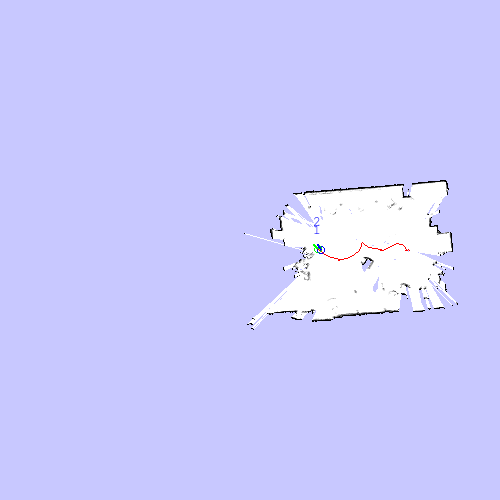
\includegraphics[width=0.5\columnwidth,keepaspectratio]{images/BadNavigation.png}
 \caption{Bad Navigation Example}
 \label{fig:BadNavigation}
\end{figure}

\subsubsection{Exploration Priority Heuristic}

By many state of the arts exploration methods, the next target of the exploring
robot is chosen by geometric features of the environment
\cite{stachniss_speeding-up_2006}. However, the room contents are not
taken into account when deciding about the room classification. For example:
a lab and a kitchen can have almost same geometric features, but they are
differed by the objects that are located in those rooms (i.e. computers, desks, 
refrigerator, coffee machine etc.). By enabling the exploring robot the ability
to distinguish different types of rooms, we can prioritize the exploration
targets. For instance: in a military operation we are likely to prefer exploring
weapon workshops rather than kitchens. 

We propose to use a vision labeler and implement the above heuristic.
After the labeler has determined current room's type, the next target will
be determined according to the priority of the type. We intend to build a
dynamic system that gets a priority set and navigates according to it. We
build on the work of \cite{sawhney_fast_2009} and propose the following weight
function of targets: $$W(x) = {p(x)} \cdot \frac {v(x)}{t(x)}$$

$x$ stands for a frontier cell. $W(x)$ stands for the weight function. $p(x)$
stands for the priority of the given cell $x$. $v(x)$ and $t(x)$ represents the
value and time which are obtained by reaching target $x$ accordingly. 
   
We claim that the above weight function represents better the reality. We
intend to test this heuristic both in simulation and real world data.


\subsubsection{Reduce Interruptions to the Operator}
\label{section:ReduceInterruptions}
An important and common task of exploring robot is to record videos of the
environment, in more praticular, to record a video for each new location (i.e.
room) that is being revealed. In current exploration methods, the robot is not
aware of its environment and therefore needs to interrupt the operator. The 
operator then manually drives the robot to a location where it records a
video. In the end of this process, the robot continues in its exploration
process and so on. In order to minimize interruptions to the operator as much
as possible, the robot should perform this common task by itself (i.e. no
interrupt the operator).

We propose to create a mechanism that analyzes whether the robot enters a room,
determines where is the best location to record the video without interrupting
the operator. In order to implement the above heuristic, we are going to base on
a semantic labeler. Rooms that are classified with the same type are likely
to have common geometric structure. Thus, the robot is likely to record those
rooms from the same location. The result is less interruptions to the operator.
Therefore, we attend to use machine learning techniques in order to learn the
best location for recording of each type. 
 
% \subsection{Corridor Detection} 
%use in order to maximize the data obtained from exploration. 
%prefer corridors instead of rooms.

% \subsection{Room Uniqueness}
% %difference between kitchen and office
% We propose to build a classifier that can distinguish between different kinds of
% rooms. For example: one can classify two different readings as rooms instead of
% corridors. Our proposed approach will classify them as two instances of the
% class room (i.e kitchen, printer-room, lab, etc.)


\section{Work Plan}
We propose to solve the problems that are mentioned above. We'll do so by:

\begin{enumerate}
 
  \item implementing IFD (Algorithm \ref{alg:IncrementalFrontierDetector}) 
  
  \item implementing a mechanism that enables the
  robot to use semantic information and speeds up the
  exploration time (section \ref{section:ExplorationScanningHeuristic})
  
  \item implementing a mechanism that enables receiving a priority set of
  scanning types and determine the targets to be explored.
  
  \item implementing a mechanism that records videos from rooms without
  interrupting the operator. This mechanism will enable to build a topological
  map of the environment. Each node will contain the video that was taken by
  the robot (\ref{section:ReduceInterruptions})
\end{enumerate}

We will test and experiment the value of each contribution of all the above
algorithms and mechanisms. We will examine the exploration speed up that is
gained by each of the proposed algorithms and mechanisms separately and all
together. 

To carry out all steps, we will use the NAO robots
in the MAVERICK research lab.
 
\begin{figure}[htb]
 \centering
 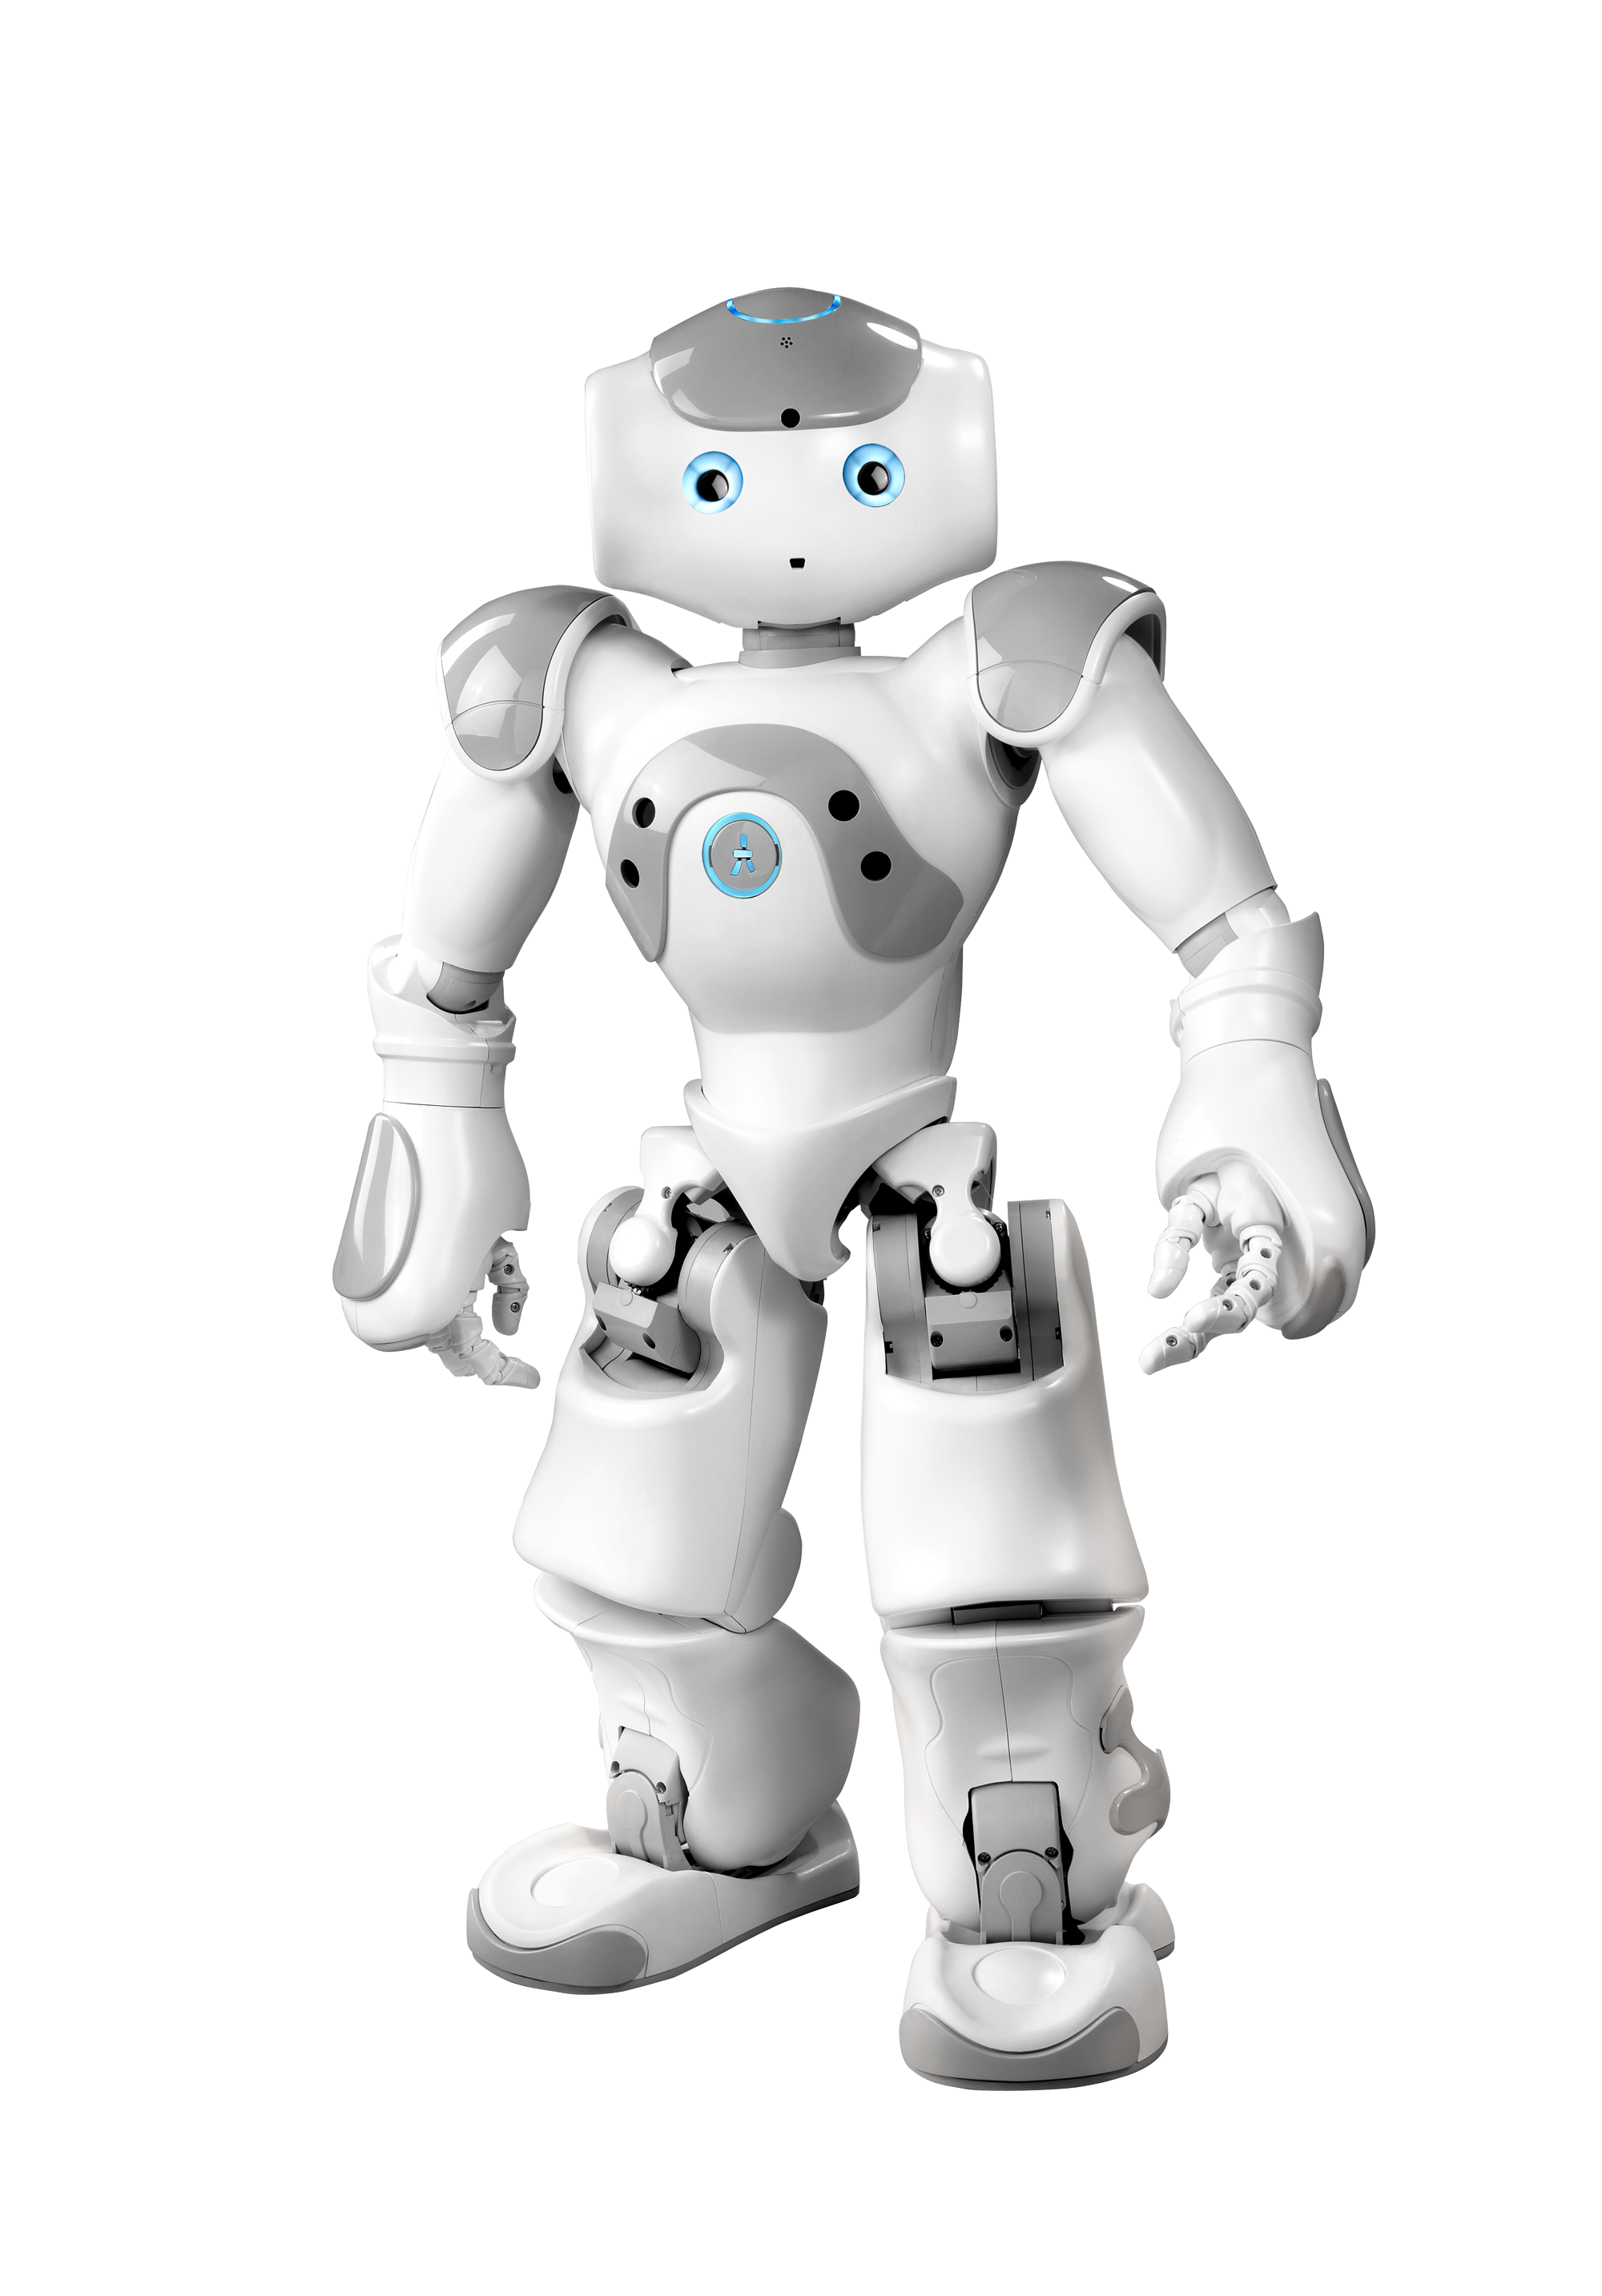
\includegraphics[width=0.5\columnwidth,keepaspectratio]{images/NAO-4_stand.png}
 \caption{NAO robot}
 \label{fig:NaoRobot}
\end{figure}

\bibliographystyle{abbrv}
\bibliography{ExplorationBib}

\end{document}
